\vspace{0.5cm}
Pour notre petit classificateur, nous allons procéder à l’entraînement de deux modèles, un modèle par classe. Chaque classe sera représentée par les ouvres des auteurs : \textit{Edgar Allan Poe} et \textit{Robert Frost}. 

\textbf{MAIS} avant de passer à l'entraînement, nous devons préparer les données afin qu'ils soient traitables pour la machine.

\vspace{0.5cm}

\textbf{Les étapes :}

\begin{enumerate}
	\item Télécharger les deux corpus
	\item Lire chaque fichier, enregistrer chaque ligne comme un objet de type \textit{list}
	\item Garder les étiquettes(1,2,...,N), une étiquette par classe.
	\item Diviser les corpus (70\% entraînement, 30\% test).
	\item Créer un \textit{mapping} (map == dict) pour associer a chaque mot unique un index numérique.
	\item Créer une boucle pour lire les lignes enregistrées dans l'objet \textit{list}
	\begin{itemize}
		\item Tokenize chaque ligne en mots (utilisez la fonction split())
	\end{itemize} 
	\item Nourrir le dictionnaire (\textit{dict}) en associant chaque mot unique à un index unique numérique.
	\item Créer un index spécial `pour les mots inconnus, des mots qui seront dans le corpus de teste mais pas dans celui d'entraînement.
	\item Changez les mots des lignes du texte par des données numériques.
	\begin{itemize}
		\item employez les index de votre dictionnaire.
		\item Créez des nouvelles listes alignées si nécessaire.
	\end{itemize}
	
\end{enumerate}



%\begin{figure}[h]
%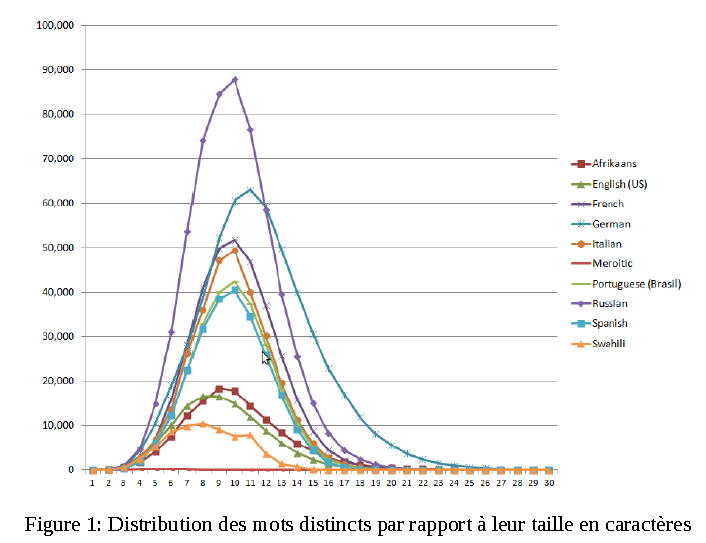
\includegraphics[width=0.6\textwidth]{../images/distrib.png}
%\caption{Distribution des mots par rapport à leur taille en caractères dans
%différentes langues\label{distrib}}
%\end{figure}

\textbf{Etape 1 : Téléchargement}

La première chose à faire consiste a télécharger les fichier qui contiennent les textes qui serviront pour entraîner et valider nos modèles. Vous pouvez trouver les fichiers aux l'adresses suivantes :

\begin{itemize}
	\item \url{https://raw.githubusercontent.com/lazyprogrammer/machine_learning_examples/master/hmm_class/edgar_allan_poe.txt}
	\item \url{https://raw.githubusercontent.com/lazyprogrammer/machine_learning_examples/master/hmm_class/robert_frost.txt}
\end{itemize}

Si vous utilisez un notebook comme \textsc{Jupyter}ou \textsc{Google Collabs}, vous pouvez utiliser le code suivant :
`
\begin{python}
	!wget -nc https://raw.githubusercontent.com/lazyprogrammer/machine_learning_examples/master/hmm_class/edgar_allan_poe.txt
	!wget -nc https://raw.githubusercontent.com/lazyprogrammer/machine_learning_examples/master/hmm_class/robert_frost.txt
\end{python}
 
\textbf{Si ça ne marche pas c'est que} : 
\begin{itemize}
\item Tout n'est pas au bon endroit (\texttt{File not Found}), regardez
dans l'onglet \texttt{files} de \textsc{Jupyter} pour voir où vous
êtes. 
\item ou que on a un problème d'encoding (\texttt{charmap}), il faut ajouter
ecoding ='utf-8' dans le open : open("13846-0.txt", encoding ="utf-8") 
\end{itemize}
Nous allons commencer par le "Discours de la Méthode", si vous avez
conservé le nom d'origine il devrait s'appeler "13846-0.txt".

\begin{python} with open("13846-0.txt") as f: chaine = f.read()
\end{python}

Et on affiche un bout du texte pour vérifier que ça marche :

\begin{python} print(chaine{[}:100{]}) \end{python}

\textbf{Etape 2 : découper}

On va très simplement découper en mots avec la \textbf{méthode} \textit{split}
\begin{python} listemots = chaine.split()\#approximation des occurrences
print("Nombre de mots : %i" %len(liste_mots))
\end{python}

\textbf{Etape 3 : compter}

On va utiliser un \textbf{dictionnaire} (ou tableau associatif) où
l'on va stocker pour chaque longueur en caractères le nombre de mots
qu'on a rencontré. Le fonctionnement est le suivant: 
\begin{itemize}
\item pour chaque mot de la liste de mots, on calcule sa longueur 
\item on vérifie si on a déjà rencontré un mot de cette longueur: 
\begin{itemize}
\item Si c'est le premier mot pour cette longueur on crée une \textbf{clé}
pour cette longueur à laquelle on affecte la \textbf{valeur} 1 
\item Sinon, on \textbf{incrémente} de 1 la valeur existante 
\end{itemize}
\end{itemize}
\begin{python} diclongueurs = {} \#un dictionnaire vide

for mot in listemots: longueur = len(mot)\#la longueur du mot if longueur
not in diclongueurs: \#on a jamais vu cette longueur de mot diclongueurs{[}longueur{]}=1
\# else: \#on a vu cette longueur de mot diclongueurs{[}longueur{]}+=1

print(diclongueurs)\#pour avoir une vue de ce qu'on a fait

\end{python}

NB: si le processus ne vous semble pas clair, ajoutez au début de
la boucle \textit{for} deux lignes (avec l'indentation) pour suivre
le processus pas à pas :

\begin{python} print(diclongueurs) dd=input("Appuyez sur Enter pour
passer a la suite") \end{python}

\textbf{Etape 4: observer}

Un dictionnaire n'est pas une structure de données ordonnée, pour
vérifier que'on trouve des résultats proche de l'attendu, on va afficher
le nombre d'occurences enregistré dans \texttt{dic\_longueurs} pour
toutes les longueurs de 1 à 30 en utilisant \textbf{l'itérateur} \textit{range}.
Dans le \textit{print} on utilise du \textbf{formatage de chaînes
de caractères}\footnote{Voir par exemple \url{https://stackoverflow.com/questions/5082452/string-formatting-vs-format}}.

\begin{python} for toto in range(1, 31):\#de 1 à 30 (31 est exclu)
nbroccurences = diclongueurs{[}toto{]} print("%i : %i"%(toto, nbr_occurences))
\end{python}

Vous verrez que le code plante car on a des longueurs qui ne sont
pas dans le dictionnaire, on va donc améliorer le code de la façon
suivante:

\begin{python} for toto in range(30): if toto in diclongueurs: nbroccurences
= diclongueurs{[}toto{]} print("%i : %i"%(toto, nbr_occurences))
 else: nbroccurences = 0 print("%i : %i"%(toto, nbr_occurences))
\end{python}

\textbf{Etape 5 : représenter}

Et maintenant c'est magique, on va créer une courbe grâce à la librairie
\texttt{matplotlib}. On va importer cette librairie et la renommer
pour que ça soit plus court à écrire. Puis pour avoir les valeurs
à mettre sur la courbe on va lire les valeurs dans l'ordre croissant
pour les ranger dans une liste nommée \textit{liste\_effectifs}. Pyplot
prend entrée un \textbf{vecteur}, une liste de valeurs ordonées.

\begin{python} import matplotlib.pyplot as pyplot \#import avec alias

listeeffectifs = {[}{]} for toto in range(30): if toto in diclongueurs:\#on
a donc vu des mots de cette longueur listeeffectifs.append(diclongueurs{[}toto{]})
else:\#on en n'a pas vu de cette longueur, on ajoute donc un 0 listeeffectifs.append(0)
pyplot.plot(listeeffectifs)\#on "dessine" pyplot.show()\#"on affiche"

\end{python}

\begin{figure}
\centering{}
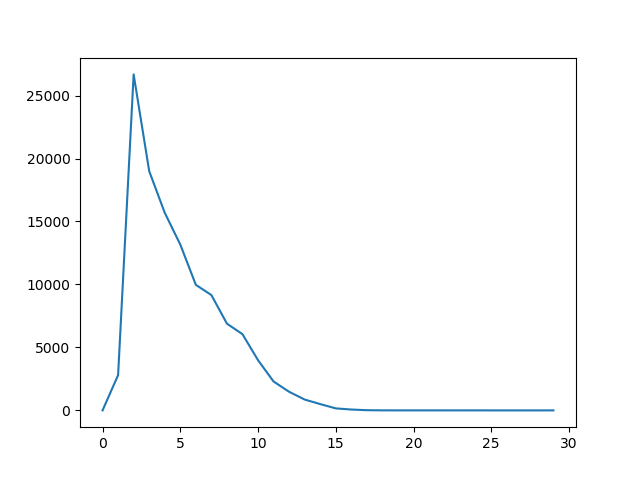
\includegraphics[width=0.5\textwidth]{../images/TD1_effectifs1.png}
\caption{"Discours de la Méthode" : nombre de mots par longueur (en abscisse),
en ordonnée l'effectif}
\end{figure}

Maintenant si on veut faire le même calcul pour l'autre texte on a
juste à changer le nom du fichier dans l'étape 1 et à relancer toutes
les cellules. Mais si on avait 100 textes à faire ça ne serait pas
très pratique. Nous allons donc voir dans l'exercice suivant comment
améliorer le code.
